Overview of \texttt{\pkg} with UML diagram.

The \texttt{view.update} package contains observer implementations that update the view. In the view, observers are primarily used for pushing concurrent updates to the view.
The package contains two kinds of observer implementations: \texttt{\lnk{SerializationObserver}} and \texttt{\lnk{ExecutionObserver}}. 
Implementations for the former update the view with a new serialized URL every time one is produced. 
Implementations for the latter update the view with a new \texttt{\lnk{LambdaTerm}} every time one is produced by the \texttt{\lnk{Executor}} and chosen to be displayed by the given \texttt{\lnk{OutputSize}}.
There are two \texttt{\lnk{SerializationObserver}} implementations:
\begin{itemize}
	\item \texttt{\lnk{UpdateShareURL}}: Updates the text panel that is opened when pressing the share button with the new URL.
	\item \texttt{\lnk{UpdateURL}}: Updates the browser URL with the new URL.
\end{itemize}
There are also two \texttt{\lnk{ExecutionObserver}} implementations:
\begin{itemize}
	\item \texttt{\lnk{UpdateUnicodeOutput}}: Updates the unicode text output panel with a new term if the panel is visible.
	\item \texttt{\lnk{UpdateTreeOutput}}: Updates the tree output panel with a new term if the panel is visible.
\end{itemize}
Both \texttt{\lnk{UpdateUnicodeOutput}} and \texttt{\lnk{UpdateTreeOutput}} use a \texttt{\lnk{Visitor}} to generate the respective \texttt{\lnk{UnicodeTerm}} and \texttt{\lnk{TreeTerm}}.
\texttt{\lnk{UnicodeTermVisitor}} is the \texttt{\lnk{Visitor}} that traverses the \texttt{\lnk{LambdaTerm}} and generates a \texttt{\lnk{UnicodeTerm}} while \texttt{\lnk{UpdateTreeOutput}} generates a \texttt{\lnk{TreeTerm}}.

\begin{figure}[H]
	\centering
	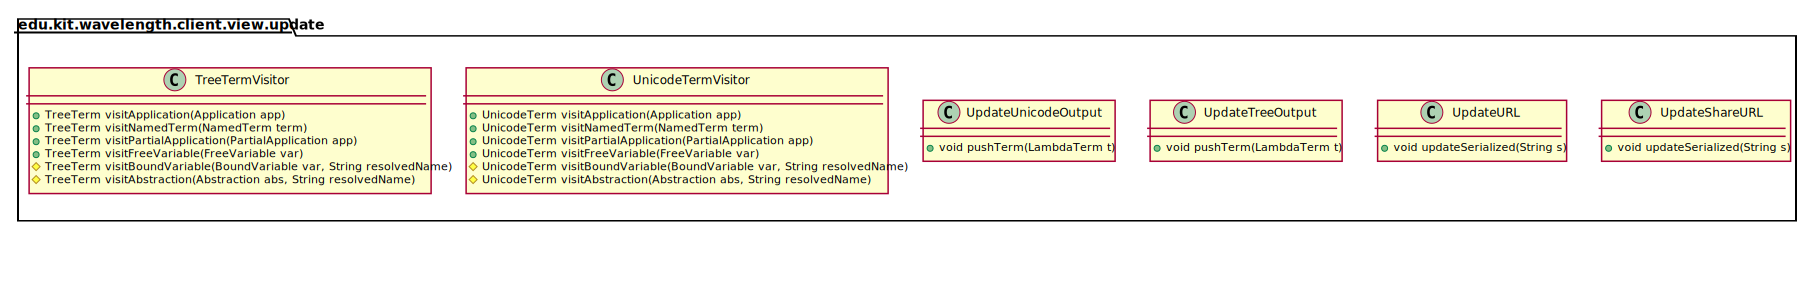
\includegraphics[width=\textwidth]{packageDiagrams/updatePackage}
\end{figure}
